% Step-by-step explainer of the order-aware (memory-contraction) models.
% Build: python make_figures.py && latexmk -pdf order_model_explainer.tex
\documentclass[11pt,a4paper]{article}
\usepackage[margin=2.3cm]{geometry}
\usepackage{lmodern}
\usepackage[T1]{fontenc}
\usepackage{microtype}
\usepackage{amsmath,amssymb}
\usepackage{graphicx}
\usepackage{booktabs}
\usepackage{xcolor}
\usepackage[hidelinks]{hyperref}
\setlength{\parindent}{0pt}
\setlength{\parskip}{6pt}

% written by make_figures.py
\newcommand{\toyGamma}{0.5}
\newcommand{\toySigmaRatio}{0.500}
\newcommand{\toySigmaFirst}{0.447}
\newcommand{\toySigmaSecond}{0.224}
\newcommand{\toySigmaNone}{0.283}
\newcommand{\toyPseFirst}{625}
\newcommand{\toyPseSecond}{447}
\newcommand{\toyPseFirstFormula}{625}
\newcommand{\toyPseSecondFormula}{447}
\newcommand{\toySigmaFirstFormula}{0.447}
\newcommand{\toySigmaSecondFormula}{0.224}
\newcommand{\toyShiftNone}{135}
\newcommand{\toyShiftFirst}{307}
\newcommand{\toyShiftSecond}{64}
\newcommand{\nUniBelow}{10}
\newcommand{\nUni}{12}
\newcommand{\nBiBelow}{63}
\newcommand{\nBi}{72}
\newcommand{\medRatioUni}{0.48}
\newcommand{\medRatioBi}{0.45}
\newcommand{\nOpposite}{18}
\newcommand{\nPse}{20}
\newcommand{\gainMin}{129}
\newcommand{\gainMax}{558}
\newcommand{\gMin}{0.40}
\newcommand{\gMax}{0.62}
\newcommand{\refMin}{304}
\newcommand{\refMax}{754}
\newcommand{\sumCausal}{-57}
\newcommand{\sumSwitching}{-108}
\newcommand{\nPids}{4}
\newcommand{\pids}{MZ, KJ, BQ, EK}
\newcommand{\checkMaxDiff}{0.0002}

% written by make_figures.py
\newcommand{\TableFits}{%
\begin{tabular}{ll rrrr}
\toprule
Participant & Model & AIC without order & AIC with order & Gain & $g$ \quad ref (ms) \\
\midrule
MZ & Forced fusion & 2490.6 & 2352.4 & -138.2 & 0.62 \quad 600 \\
 & Causal inference & 2480.4 & 2337.4 & -143.0 & 0.61 \quad 604 \\
 & Cue switching & 2488.7 & 2359.5 & -129.3 & 0.58 \quad 598 \\
\addlinespace
KJ & Forced fusion & 2405.0 & 2121.0 & -283.9 & 0.42 \quad 419 \\
 & Causal inference & 2405.3 & 2118.1 & -287.2 & 0.43 \quad 420 \\
 & Cue switching & 2400.5 & 2097.3 & -303.2 & 0.40 \quad 423 \\
\addlinespace
BQ & Forced fusion & 2807.8 & 2560.6 & -247.1 & 0.59 \quad 316 \\
 & Causal inference & 2793.6 & 2534.1 & -259.6 & 0.61 \quad 304 \\
 & Cue switching & 2792.2 & 2505.1 & -287.1 & 0.54 \quad 344 \\
\addlinespace
EK & Forced fusion & 2494.7 & 1937.1 & -557.6 & 0.61 \quad 754 \\
 & Causal inference & 2482.5 & 1924.4 & -558.1 & 0.61 \quad 747 \\
 & Cue switching & 2459.3 & 1901.1 & -558.2 & 0.57 \quad 722 \\
\addlinespace
\bottomrule
\end{tabular}}
\newcommand{\TableComparison}{%
\begin{tabular}{l rr}
\toprule
Participant & Causal inference & Cue switching \\
\midrule
MZ & -14.9 & +7.1 \\
KJ & -3.0 & -23.7 \\
BQ & -26.6 & -55.5 \\
EK & -12.7 & -36.0 \\
\midrule
Summed & -57.2 [-92, -24] & -108.1 [-190, -15] \\
\bottomrule
\end{tabular}}


\newsavebox{\keyboxbin}
\newenvironment{keybox}[1][]%
  {\def\kbtitle{#1}\setlength{\fboxsep}{7pt}\begin{lrbox}{\keyboxbin}%
   \begin{minipage}{\dimexpr\linewidth-2\fboxsep-2\fboxrule\relax}%
   \ifx\kbtitle\empty\else{\bfseries\kbtitle}\par\fi}%
  {\end{minipage}\end{lrbox}\par\medskip\noindent
   \fcolorbox{blue!40!black}{blue!3}{\usebox{\keyboxbin}}\par\medskip}
\newcommand{\step}[1]{\section{#1}}

\title{Presentation order in the duration task:\\the memory-contraction model, step by step}
\author{av-dur-estimation, v2 analysis (exploratory)}
\date{19 November 2026}

\begin{document}
\maketitle

\begin{keybox}[In short]
\begin{itemize}
  \item People are much more precise when the test comes \emph{second}, and their bias flips sign
        between the two orders. None of our three models (fusion, causal inference, switching) can
        produce this, because they treat the two intervals the same.
  \item A noisier first interval does not explain it either (Step~4).
  \item What does explain it: the first interval has to be held in memory, and memory pulls it toward a
        typical duration. Two parameters: how much of the first interval survives ($g$) and what it is
        pulled toward (ref).
  \item Added to all three models, this improves the fit by \gainMin--\gainMax{} AIC points per
        participant, for 2 extra parameters. With order in the models, causal inference and switching both
        beat fusion; switching leads (summed $\Delta$AIC \sumSwitching{} against \sumCausal{}).
  \item Exploratory: \nPids{} participants (\pids), no recovery check yet. Code:
        \texttt{avdur\_analysis/order\_models.py}; notebook \texttt{04\_order\_models.ipynb}.
\end{itemize}
\end{keybox}

%──────────────────────────────────────────────────────────────────────────────
\step{The task and the two orders}

Every trial has two intervals. One is the \emph{standard}: 500\,ms of sound, plus in the main experiment
a light whose duration differs from the sound by the conflict ($-450$ to $+450$\,ms). The other is the
\emph{test}: sound and light of the same duration, which the staircases vary. The participant says which
interval was longer.

The order is random: on half the trials the test comes first, on the other half second
(Figure~\ref{fig:schematic}A). Until now we pooled the two orders.

\begin{figure}[h]
  \centering
  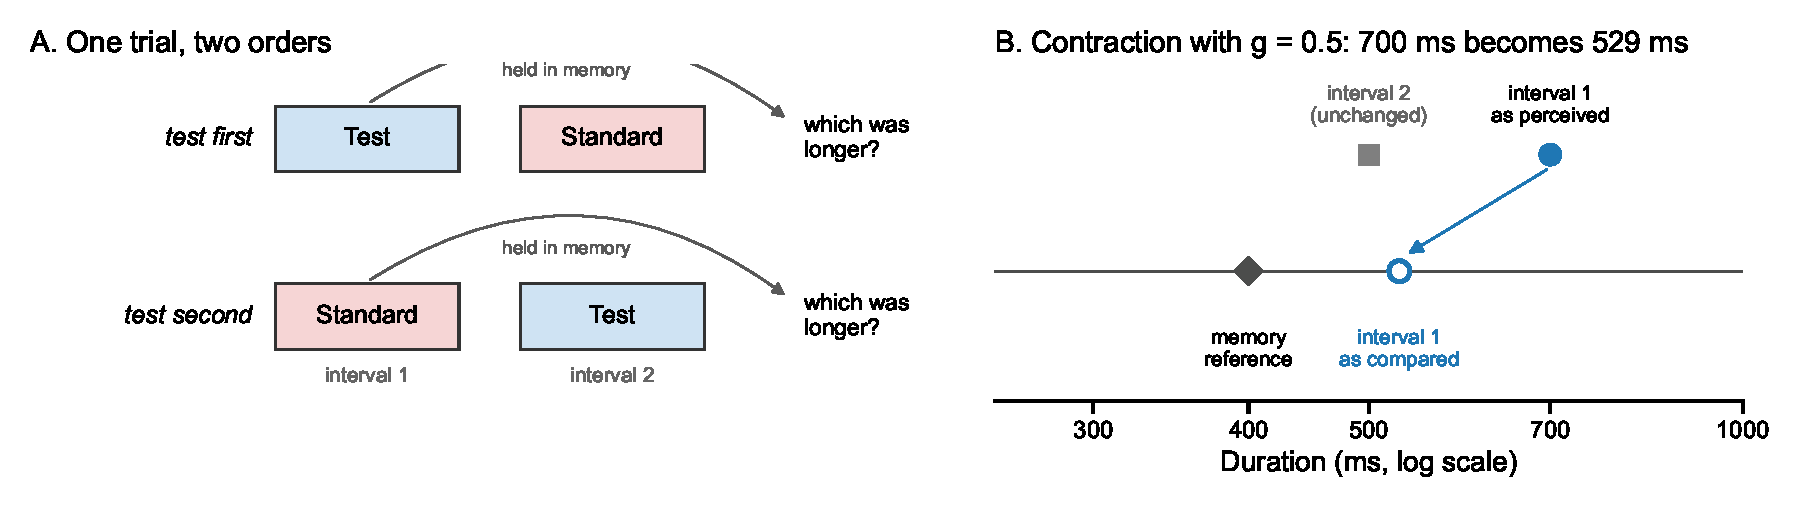
\includegraphics[width=\linewidth]{figures/fig1_schematic.pdf}
  \caption{\textbf{A.} The two orders. Whichever interval comes first has to be remembered until the
  second one ends. \textbf{B.} Memory contraction: the first interval (here perceived as 700\,ms) is
  pulled toward a remembered reference (400\,ms) before the comparison; with $g = 0.5$ it is compared as
  if it lasted 529\,ms. The second interval is used as perceived.}
  \label{fig:schematic}
\end{figure}

%──────────────────────────────────────────────────────────────────────────────
\step{What the models assumed so far}

All models work on log duration. In each interval the observer gets a noisy measurement $m$ of the true
log duration, with noise $\sigma$ (auditory, visual, or both). From the measurements of one interval the
model forms an \emph{estimate} $e$ of how long that interval was:
\begin{itemize}
  \item \textbf{forced fusion}: a reliability-weighted average of the sound and the light;
  \item \textbf{cue switching}: on each interval, either the sound or the light, at random;
  \item \textbf{causal inference}: a mix of the two, depending on how likely it is that both came from
        one event.
\end{itemize}
The answer is ``test longer'' when $e_\text{test} > e_\text{standard}$ (apart from occasional lapses). In
that rule the two intervals are interchangeable, so \emph{the order cannot matter}: test-first and
test-second trials have the same psychometric curve.

%──────────────────────────────────────────────────────────────────────────────
\step{What the data show}

Fitting the psychometric curve separately for test-first and test-second trials
(Figure~\ref{fig:evidence}):
\begin{itemize}
  \item \textbf{Precision.} The curve is steeper (smaller $\sigma$) with the test second in
        \nUniBelow{} of \nUni{} unimodal conditions and \nBiBelow{} of \nBi{} bimodal conditions. The
        median ratio $\sigma_\text{second}/\sigma_\text{first}$ is \medRatioUni{} (unimodal) and
        \medRatioBi{} (bimodal): with the test first, $\sigma$ is about twice as large.
  \item \textbf{Bias.} The PSE shifts in opposite directions for the two orders in \nOpposite{} of
        \nPse{} cases. Its direction differs between people: KJ and BQ need a longer test when it comes
        first, EK and (mostly) MZ a shorter one.
  \item \textbf{Visual too.} The effect is as clear in the visual block as in the auditory ones, so it is
        not about the sound or its noise.
\end{itemize}

\begin{figure}[h]
  \centering
  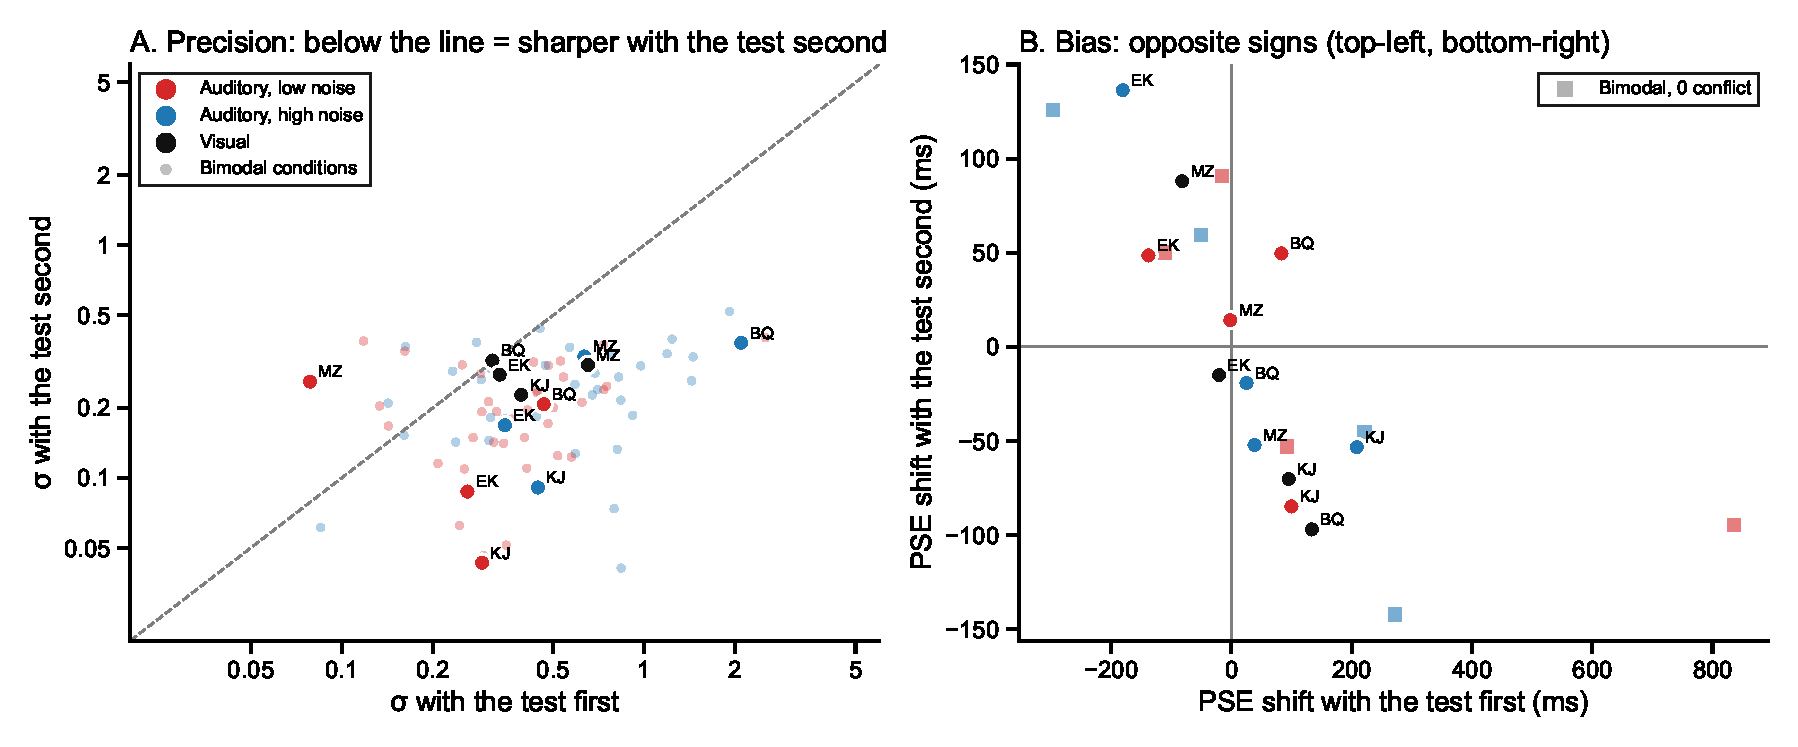
\includegraphics[width=\linewidth]{figures/fig3_evidence.pdf}
  \caption{Order effects in the data (\pids). \textbf{A.} Psychometric $\sigma$ with the test first
  ($x$) and second ($y$); large dots: unimodal blocks, small dots: bimodal conditions. Almost everything
  lies below the diagonal. \textbf{B.} PSE shift with the test first and second (unimodal blocks, and the
  bimodal conditions without conflict): mostly opposite signs.}
  \label{fig:evidence}
\end{figure}

%──────────────────────────────────────────────────────────────────────────────
\step{A first idea that does not work: a noisier first interval}

Perhaps the first interval is just measured less precisely, with noise $\sigma_1 > \sigma_2$. Ignore
the prior for a moment, so the estimate is the measurement. Then
\[
  P(\text{test longer}) =
  \Phi\!\left(\frac{\log t - \log s}{\sqrt{\sigma_1^2 + \sigma_2^2}}\right)
  \quad\text{for \emph{both} orders,}
\]
with $t$ the test and $s$ the standard duration. The comparison noise is
$\sqrt{\sigma_1^2+\sigma_2^2}$ whichever interval holds the test, so the curves are identical: no
difference in slope, no bias. This idea is out.

%──────────────────────────────────────────────────────────────────────────────
\step{Memory contraction}

The first interval is over before the second starts, so it must be remembered. A well-known finding in
time perception is that remembered durations drift toward the typical duration of the experiment
(central tendency, or ``Vierordt's law''). For two-interval tasks this was formalised by Dyjas,
Bausenhart and Ulrich (2012) as the \emph{internal reference model}: the first interval is blended with a
remembered reference before the comparison. In our notation:
\begin{keybox}
\[
  e_1' \;=\; g\, e_1 + (1-g)\,\text{ref}, \qquad e_2' = e_2 .
\]
\begin{itemize}
  \item $e_1, e_2$: the model's estimates of interval 1 and 2 (fusion, switching or causal inference, or
        the single cue in the unimodal blocks), exactly as before.
  \item $g$ (\texttt{g\_first}, between 0 and 1): how much of the first interval survives.
        $g = 1$: no contraction, the old models. $g = 0.5$: half the first interval, half the reference.
  \item ref: the reference it is pulled toward (log duration; we report it in ms).
\end{itemize}
\end{keybox}
Only the first interval is contracted, so the order now matters: on test-first trials the
\emph{test} is contracted, on test-second trials the \emph{standard} is.

%──────────────────────────────────────────────────────────────────────────────
\step{What contraction predicts}

Again ignoring the prior, with noise $\sigma$ per interval, and the standard's own estimate centred at
$\log s + \Delta$ ($\Delta$ is how far the light pulls the standard; $\Delta = 0$ in the unimodal blocks):

\textbf{Test first.} ``Test longer'' when $g\,m_t + (1-g)\,\text{ref} > m_s$, so
\[
  \sigma_\text{first} = \frac{\sqrt{1+g^2}}{g}\,\sigma, \qquad
  \log \text{PSE}_\text{first} = \frac{\log s + \Delta - (1-g)\,\text{ref}}{g}.
\]
\textbf{Test second.} ``Test longer'' when $m_t > g\,m_s + (1-g)\,\text{ref}$, so
\[
  \sigma_\text{second} = \sqrt{1+g^2}\,\sigma, \qquad
  \log \text{PSE}_\text{second} = g\,(\log s + \Delta) + (1-g)\,\text{ref}.
\]

Three predictions follow, one for each pattern in the data:
\begin{enumerate}
  \item \textbf{Precision:} $\sigma_\text{second} / \sigma_\text{first} = g$. The test-second curve is
        steeper. A ratio of about 0.5 in the data means $g \approx 0.5$.
  \item \textbf{Bias:} without conflict, the PSE moves by $(1-g)(\log s - \text{ref})/g$ with the test
        first and by $(1-g)(\text{ref} - \log s)$ with the test second: \emph{opposite signs}. Which way
        depends on whether ref is below or above 500\,ms, so it can differ between people.
  \item \textbf{Conflict effect:} the light's pull $\Delta$ shows up as $\Delta/g$ with the test first
        and as $g\,\Delta$ with the test second. With the test second, the conflict barely moves the PSE;
        with the test first, it moves it a lot.
\end{enumerate}

Figure~\ref{fig:toy} shows this with made-up values. The model code reproduces the formulas: with
$\sigma = 0.2$, $g = \toyGamma$ and ref = 400\,ms it gives $\sigma_\text{first} = \toySigmaFirst$ and
$\sigma_\text{second} = \toySigmaSecond$ (formulas: \toySigmaFirstFormula{} and
\toySigmaSecondFormula), and PSEs of \toyPseFirst{} and \toyPseSecond\,ms (formulas:
\toyPseFirstFormula{} and \toyPseSecondFormula\,ms). In panel~B, a +250\,ms conflict moves the PSE
by \toyShiftNone\,ms without contraction, by \toyShiftFirst\,ms with the test first and by
\toyShiftSecond\,ms with the test second (about $\times 2$ and $\times 0.5$; not exactly, because the
plot is in ms rather than log units).

\begin{figure}[h]
  \centering
  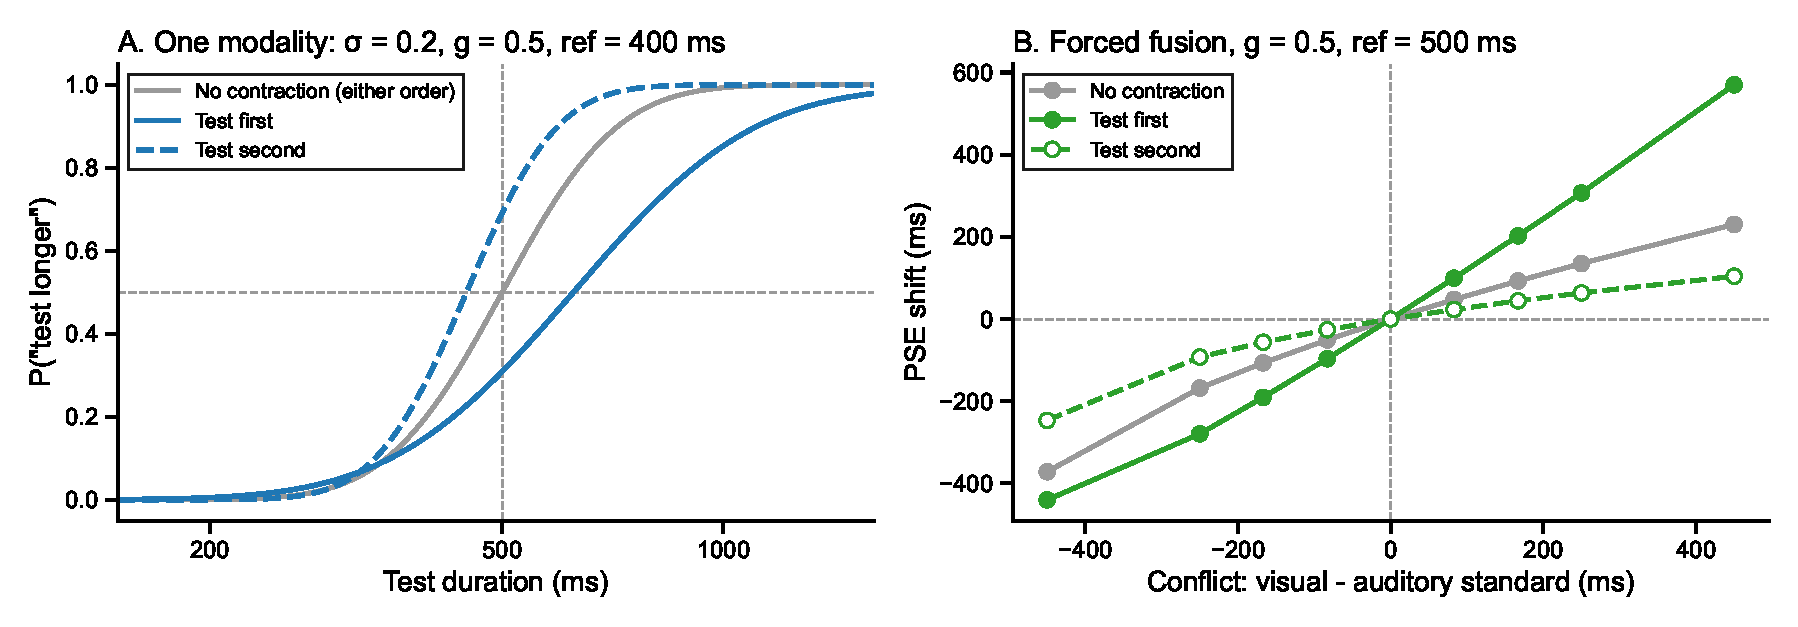
\includegraphics[width=\linewidth]{figures/fig2_predictions_toy.pdf}
  \caption{Contraction with made-up values. \textbf{A.} One modality: the test-first curve is flatter
  and shifted right, the test-second curve steeper and shifted left (ref = 400\,ms, below the
  standard). \textbf{B.} Forced fusion in the main experiment, with ref = 500\,ms so that only the
  conflict effect changes: larger with the test first, smaller with the test second.}
  \label{fig:toy}
\end{figure}

\textbf{Why this matters for the old fits.} Pooling the two orders mixes a flat curve and a steep one
shifted in opposite directions. The pooled curve is flatter than either, and its conflict effect is an
average of $\Delta/g$ and $g\Delta$. The order-free models then have to bend their noise parameters to
match. For example, KJ's fusion fit needed a visual $\sigma$ more than three times larger than KJ's visual
block shows (0.69 against about 0.20).

%──────────────────────────────────────────────────────────────────────────────
\step{Putting contraction into the three models}

Each model keeps its own estimate and its own parameters; contraction is applied to whichever interval
comes first, in every block (unimodal auditory, unimodal visual, main experiment). Per participant:
\begin{center}
\begin{tabular}{ll}
  \toprule
  All models & lapse, $\sigma_A$ (low noise), $\sigma_A$ (high noise), $\sigma_V$, \textbf{g, ref} \\
  Causal inference & $+\,p_c$ \\
  Cue switching & $+\,p_\text{switch}$ (low noise), $p_\text{switch}$ (high noise) \\
  \bottomrule
\end{tabular}
\end{center}
$g$ and ref are shared by all blocks and conditions. That is the simplest choice and an assumption
(Step~11).

%──────────────────────────────────────────────────────────────────────────────
\step{How the likelihood is computed (no simulation)}

For one interval, every model gives a full distribution of the estimate $e$. We compute its cumulative
distribution $F(e)$ on a grid of 1500 durations between 50 and 2000\,ms (the prior range):
\begin{itemize}
  \item \textbf{unimodal blocks and fusion}: exactly, by inverting the estimate (the prior-truncated mean
        is an increasing function of the measurement);
  \item \textbf{switching}: the mixture of the auditory and visual distributions;
  \item \textbf{causal inference}: the same quadrature as in the main models.
\end{itemize}
Contraction is a stretch-and-shift of the first interval's estimate, so
\[
  P(\text{test longer}) = \sum_{y} \Bigl[1 - F_\text{test}\bigl(\varphi(y)\bigr)\Bigr]\,
  \Delta F_\text{standard}(y),
  \qquad
  \varphi(y) =
  \begin{cases}
    \bigl(y - (1-g)\,\text{ref}\bigr)/g & \text{test first,}\\[2pt]
    g\,y + (1-g)\,\text{ref} & \text{test second,}
  \end{cases}
\]
one sum over the grid per stimulus pair. Then come the lapse and a binomial likelihood over every
(block, noise, conflict, test duration, order) cell. Fits use L-BFGS-B from 6 starts. A fit takes 2--4
minutes per participant for fusion and switching and 8--15 for causal inference.

%──────────────────────────────────────────────────────────────────────────────
\step{Checks}
\begin{itemize}
  \item \textbf{$g = 1$ gives the old models.} At the main fits' parameters, the order code reproduces
        their $-\log L$ for all three models (largest difference \checkMaxDiff).
  \item \textbf{Against simulation.} For all three models and both orders, the computed probabilities
        match 400{,}000 simulated trials to within 0.002 (simulation error).
  \item \textbf{Against the formulas.} Step~6: the code reproduces the closed-form $\sigma$ and PSE
        values.
\end{itemize}

%──────────────────────────────────────────────────────────────────────────────
\step{Results}

\textbf{Contraction helps every model, a lot.} Adding $g$ and ref lowers AIC by \gainMin--\gainMax{}
points per participant (Table~\ref{tab:fits}, Figure~\ref{fig:summary}A). Two parameters are worth only
4 AIC points, so this is far beyond what the extra freedom alone could buy.

\textbf{The parameters are consistent.} $g$ lies between \gMin{} and \gMax{}: about half of the first
interval survives. The three models agree on $g$ and ref for each person
(Figure~\ref{fig:summary}C--D). ref ranges from \refMin{} to \refMax\,ms. Its position relative to
500\,ms predicts the direction of each person's bias: KJ and BQ (ref below 500\,ms) need a longer test
when it comes first, and EK and, mostly, MZ (ref above 500\,ms) a shorter one, as in Figure~\ref{fig:evidence}B.

\begin{table}[h]
  \centering\small
  \TableFits
  \caption{Fits with and without order. Gain: AIC with order minus without (negative: order helps).}
  \label{tab:fits}
\end{table}

\textbf{Model comparison with order} (Table~\ref{tab:comparison}, Figure~\ref{fig:summary}B). Causal
inference now beats fusion in every participant, and switching beats it in three of four (MZ prefers
causal inference). Summed over participants, switching leads; both intervals, from resampling the four
participants, stay below zero.

\begin{table}[h]
  \centering\small
  \TableComparison
  \caption{$\Delta$AIC against forced fusion, all models with contraction (negative: better than
  fusion). Summed: with a 95\% interval from resampling participants.}
  \label{tab:comparison}
\end{table}

\begin{figure}[tbp]
  \centering
  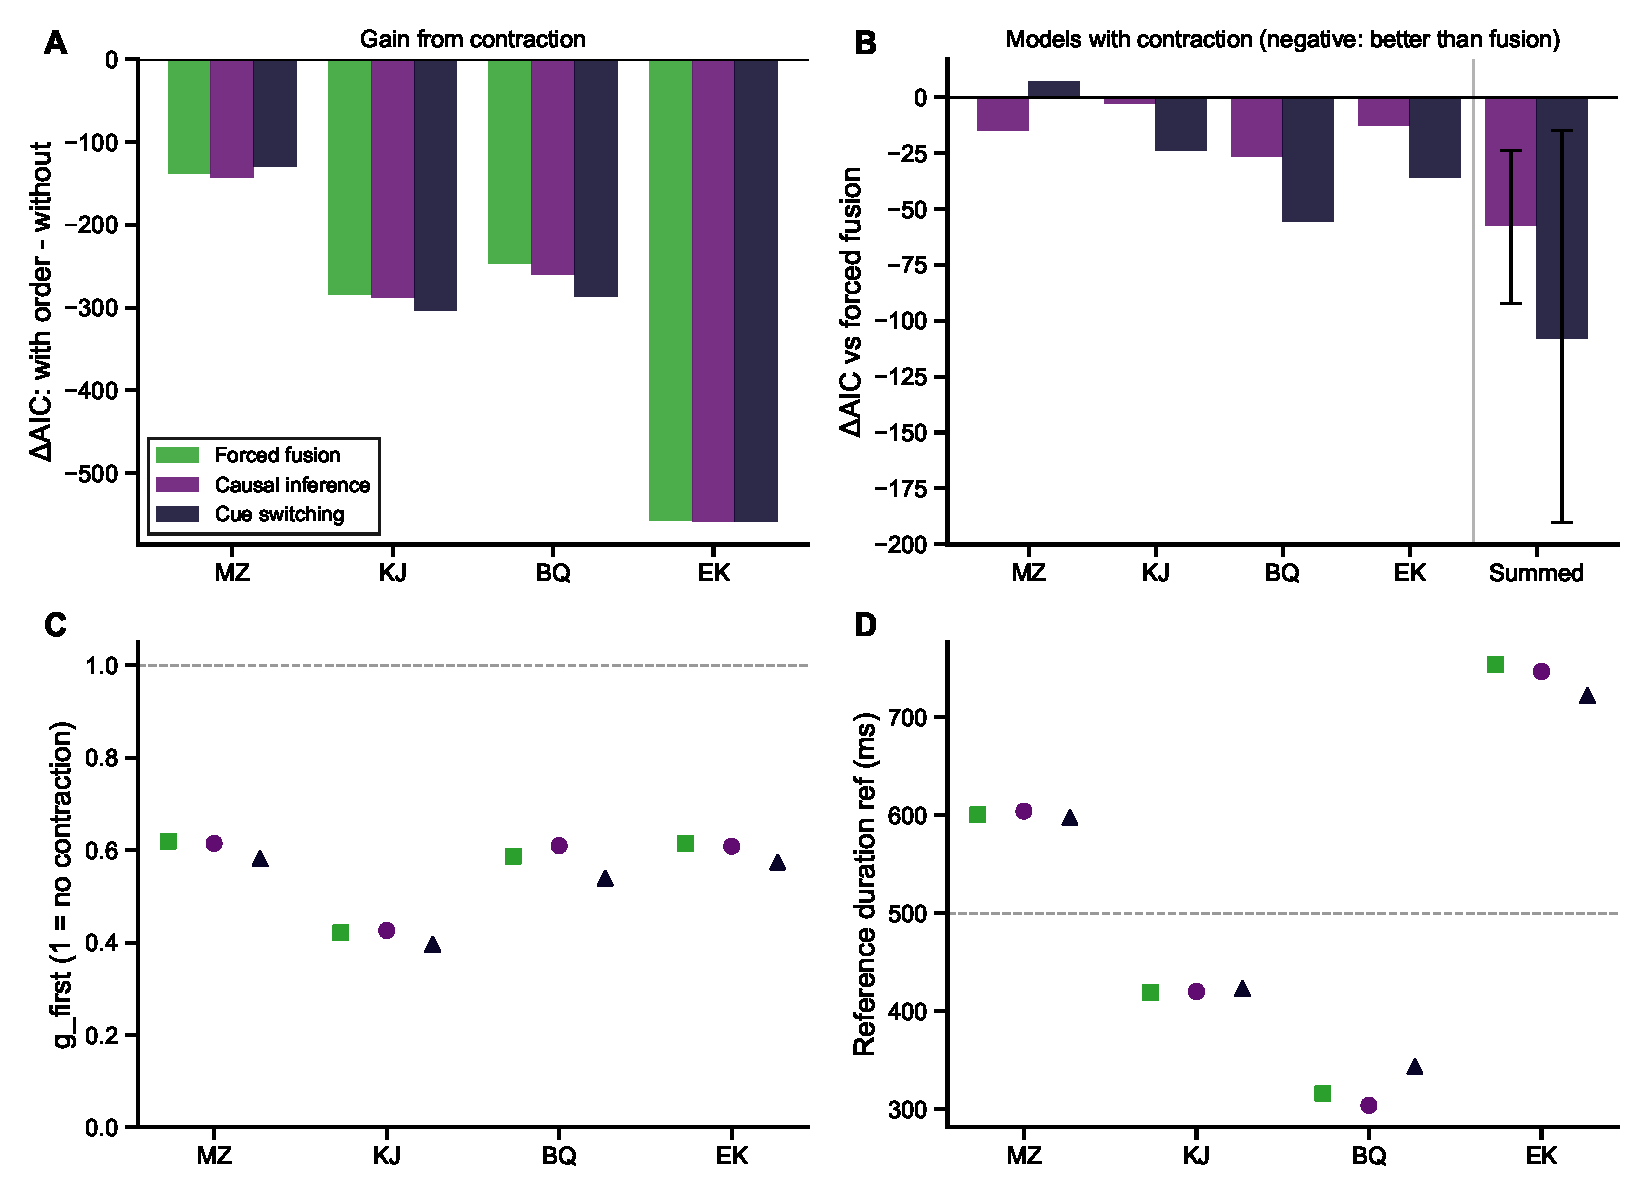
\includegraphics[width=0.85\linewidth]{figures/fig4_fit_summary.pdf}
  \caption{\textbf{A.} AIC gain from contraction for each model. \textbf{B.} Models with contraction
  against forced fusion. \textbf{C.} Fitted $g$ (1 = no contraction). \textbf{D.} Fitted reference
  duration; dashed: the 500\,ms standard.}
  \label{fig:summary}
\end{figure}

\begin{figure}[tbp]
  \centering
  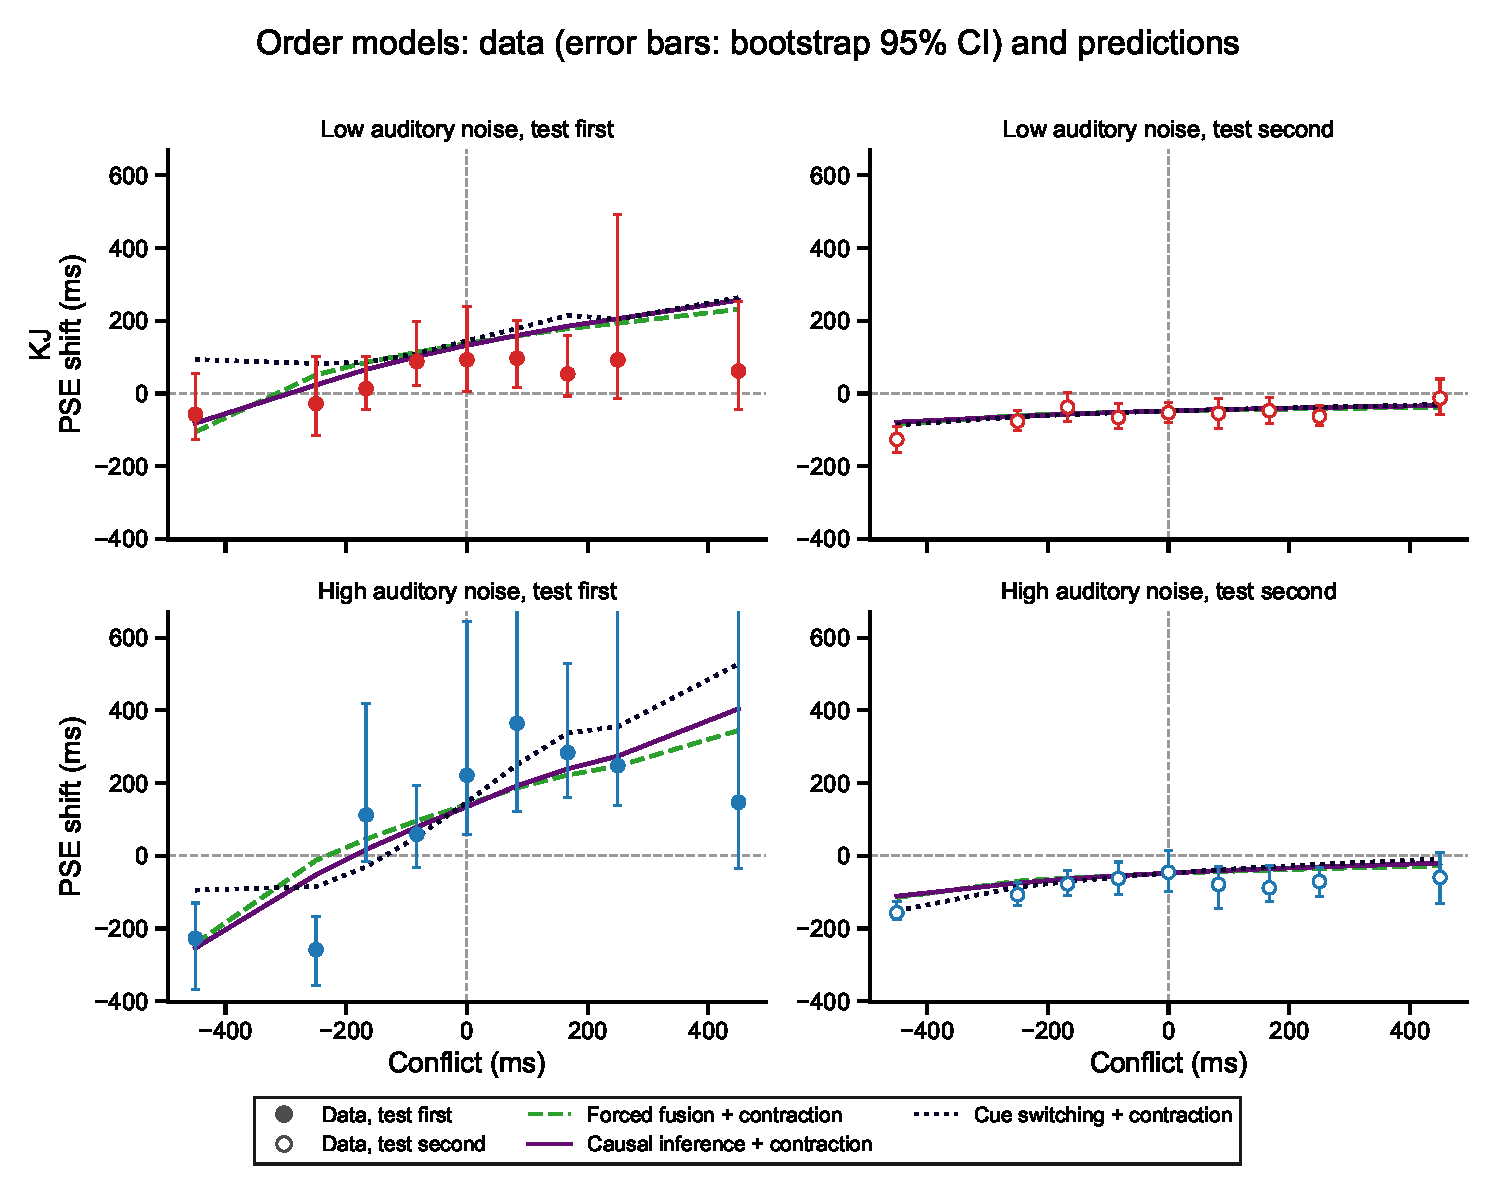
\includegraphics[width=0.8\linewidth]{figures/fig5_predictions_KJ.pdf}
  \caption{KJ: data (points, bootstrap 95\% intervals) and predictions of the three models with
  contraction (lines); rows: noise level, columns: order. The test-first curves (left) follow the
  conflict steeply; the test-second curves (right) hardly move. This is the
  pattern behind KJ's missing bias at +450\,ms in the pooled data.}
  \label{fig:kj}
\end{figure}

\begin{figure}[tbp]
  \centering
  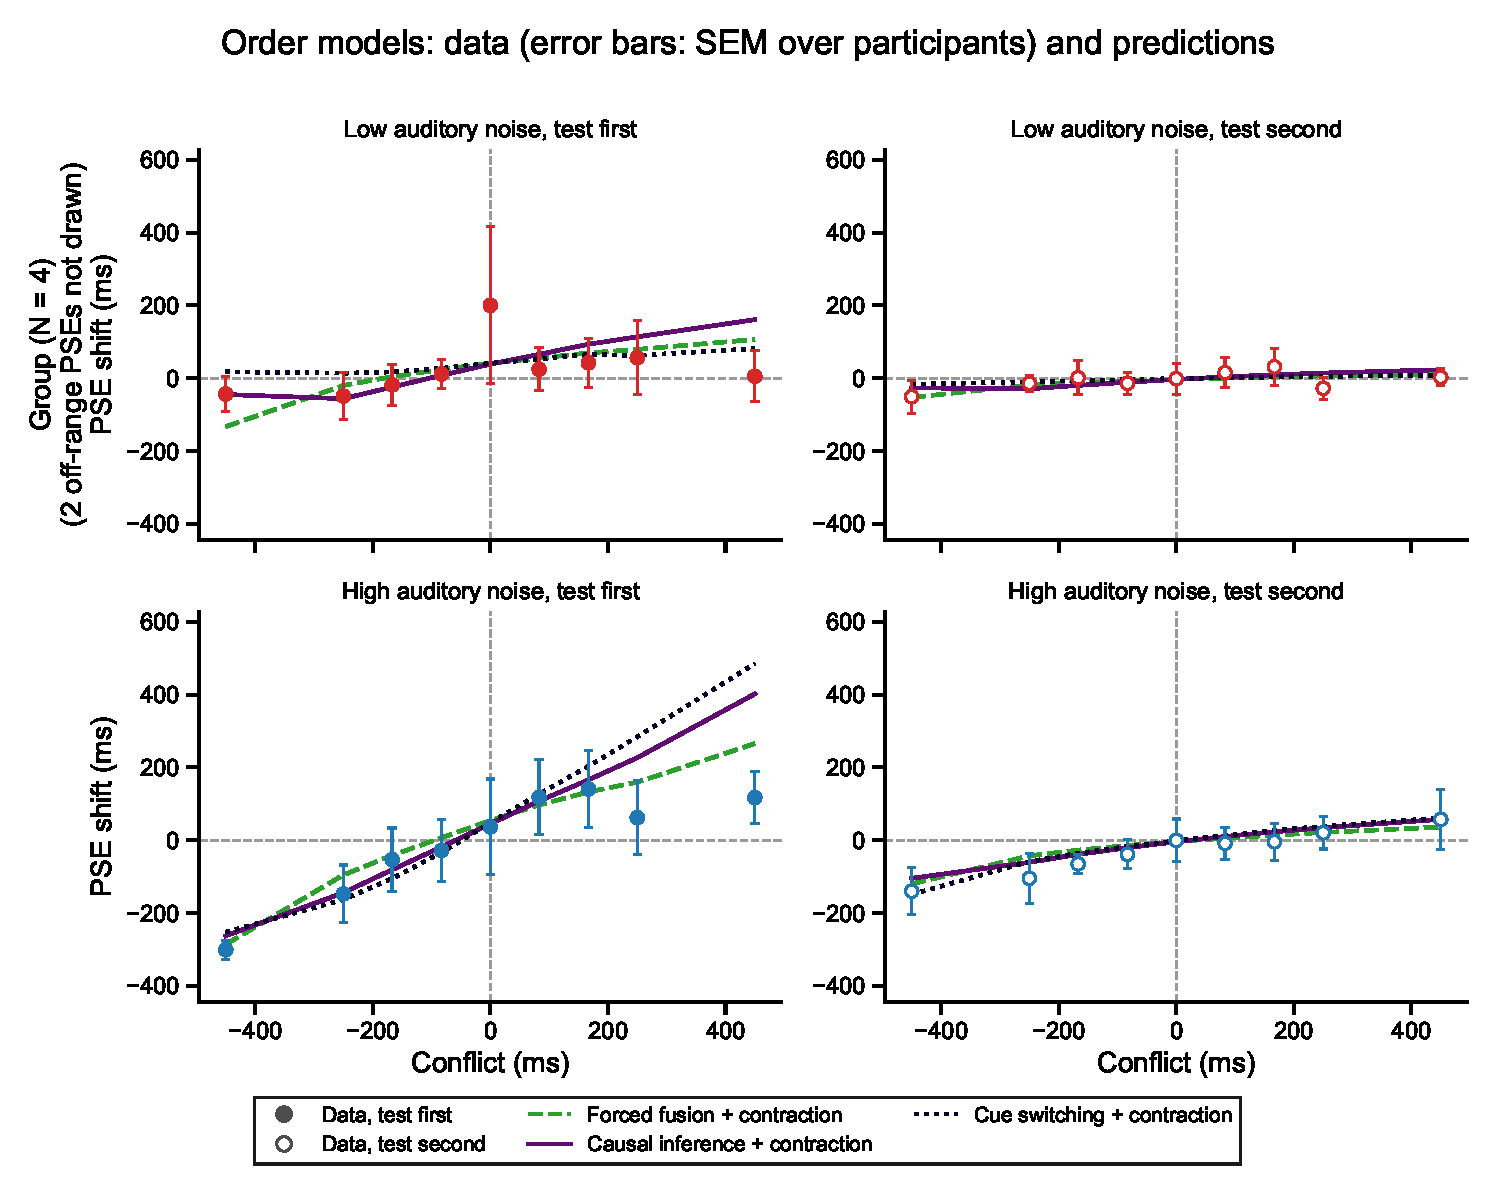
\includegraphics[width=0.8\linewidth]{figures/fig6_predictions_group.pdf}
  \caption{Group (mean $\pm$ SEM over participants) and the models' mean predictions. Two test-first
  PSEs of BQ lie outside the tested durations and are left out.}
  \label{fig:group}
\end{figure}

\textbf{KJ again.} With contraction, KJ's puzzle goes away (Figure~\ref{fig:kj}). KJ's $g$ is about 0.4,
so on test-second trials the conflict moves the PSE only about 0.4 times as far. On test-first trials it
moves it about 2.5 times as far, but those estimates are very uncertain. Pooled, the large +450\,ms
conflict ended up with almost no bias.

%──────────────────────────────────────────────────────────────────────────────
\step{What this means, and what is not settled}

\begin{itemize}
  \item \textbf{Order belongs in the models.} The improvement is large and the same in every person and
        model. It also answers reviewer~1's question on presentation order with a mechanism, not only a
        split analysis.
  \item \textbf{The model ranking holds up.} With order in, causal inference and switching both beat
        fusion, now in all or nearly all participants. Switching still leads, but with four
        participants that is not settled.
  \item \textbf{Assumptions to discuss with the PI:}
    \begin{itemize}
      \item \emph{Shared $g$ and ref across blocks.} The unimodal and bimodal blocks could differ; a
            per-block $g$ would test that.
      \item \emph{Free ref.} ref could instead be tied to something fixed, such as the middle of the
            tested range, saving a parameter.
      \item \emph{Alternatives.} A simple time-order bias (an additive shift for the first interval)
            would explain the opposite PSE shifts but not the change in precision. It is worth fitting as
            a competitor.
      \item \emph{Meaning of $\sigma$.} $\sigma_A$ and $\sigma_V$ are now the noise of an interval
            \emph{before} memory, so they are smaller than in the order-free fits and not directly
            comparable with them.
    \end{itemize}
  \item \textbf{Not done yet:} parameter and model recovery for the order models, the
        free-visual-weight model with order, and more participants.
\end{itemize}

\vspace{1em}
\textbf{Reference.} Dyjas, O., Bausenhart, K.~M., \& Ulrich, R. (2012). Trial-by-trial updating of an
internal reference in discrimination tasks: Evidence from effects of stimulus order and trial sequence.
\emph{Attention, Perception, \& Psychophysics}, 74(8), 1819--1841.

\end{document}
